%yright 2007, 2008, 2009 Elsevier Ltd
%% 
%% This file is part of the 'Elsarticle Bundle'.
%% ---------------------------------------------
%% 
%% It may be distributed under the conditions of the LaTeX Project Public
%% License, either version 1.2 of this license or (at your option) any
%% later version.  The latest version of this license is in
%%    http://www.latex-project.org/lppl.txt
%% and version 1.2 or later is part of all distributions of LaTeX
%% version 1999/12/01 or later.
%% 
%% The list of all files belonging to the 'Elsarticle Bundle' is
%% given in the file `manifest.txt'.
%% 

%% Template article for Elsevier's document class `elsarticle'
%% with numbered style bibliographic references
%% SP 2008/03/01

% \documentclass[preprint,11pt]{elsarticle}
\documentclass[final,1p,11pt]{elsarticle}

%\documentclass[final,1p,times]{elsarticle}


%% Use the option review to obtain double line spacing
%%\documentclass[authoryear,preprint,review,12pt]{elsarticle}

%% Use the options 1p,twocolumn; 3p; 3p,twocolumn; 5p; or 5p,twocolumn
%% for a journal layout:
%% \documentclass[final,1p,times]{elsarticle}
%% \documentclass[final,1p,times,twocolumn]{elsarticle}
%% \documentclass[final,3p,times]{elsarticle}
%% \documentclass[final,3p,times,twocolumn]{elsarticle}
%% \documentclass[final,5p,times]{elsarticle}
%% \documentclass[final,5p,times,twocolumn]{elsarticle}

%%% For including figures, graphicx.sty has been loaded in
%% elsarticle.cls. If you prefer to use the old commands
%% please give \usepackage{epsfig}


\usepackage{epsfig}
%\usepackage{cite}
%\usepackage{mcite}
\usepackage{array,tabularx,epsfig,mathrsfs,graphicx,rotating}
\usepackage{ifthen}
\usepackage{amsfonts}
\usepackage{ragged2e}
\PassOptionsToPackage{hyphens}{url}
\usepackage[hyphens]{url}
\usepackage{hyperref}
\usepackage{listings}
\usepackage{subfigure}
\usepackage{epstopdf}
% Custom colors
\usepackage{color}
\usepackage{float}

% to cross text
\usepackage[normalem]{ulem} % either use this (simple) or
\usepackage{soul} % use this (many fancier options)


\hypersetup{
  colorlinks=true,
  linkcolor=blue,
  citecolor=blue,
  urlcolor=blue
}




\graphicspath{{figs/}}


\pdfinfo{
   /Author (Chekanov/Demarteau)
   /Title  (Conceptual Design Studies for a CEPC Detector)
   /CreationDate (D:20160102195600)
   /Subject (PDFLaTeX)
   /Keywords (PDF;LaTeX)
}


\textheight=22cm
\textwidth=14.5cm

\newcommand{\beq}{\begin{equation}}
\newcommand{\eeq}{\end{equation}}
\newcommand{\la}{\langle}
\newcommand{\promc}{{\sc ProMC}}
\newcommand{\ra}{\rangle}
\newcommand{\eps}{\epsilon}
\newcommand{\ud}{\mathrm{d}}
\newcommand{\Ec}{\mathcal{E}}
\newcommand{\Fc}{\mathcal{F}}
\newcommand{\Za}{\mathrm{Z_1}}
\newcommand{\Zb}{\mathrm{Z_2}}
\newcommand{\Zn}{\mathrm{Z_n}}
\newcommand{\F}{\mathrm{F}}

\chardef\til=126
\newcommand{\mev}{{\,\mathrm{MeV}}}
\newcommand{\gev}{{\,\mathrm{GeV}}}
\newcommand{\tev}{{\,\mathrm{TeV}}}
\newcommand{\GEANTfour} {\textsc{geant4}}
\journal{XXX-XXX}



\begin{document}

\section*{Another study about the c variables}
%In the past paper~\cite{Larkoski:2013eya}, It mention that in some process at $c_2$, when $\beta=1.7$, it will have the best separation power. We try to use this in our study to see whether it is suitable for our research.\\

%In Figure \textcolor{blue}{9},\textcolor{blue}{1}0 and \textcolor{blue}{11}, they are the ROC curves of the different $\beta$ quantities in $c_2$ at different energies of collision. We can see that in all cell sizes, separation power isn't improved by increasing $\beta$ quantity to 1.7. We can see from $\beta=1$ to $\beta=2$, the separation power is worse and worse in all cell sizes in all energies of collision.\\

In Reference~\cite{Larkoski:2013eya}, it is said that the $c_2$ will have the best separation power when $\beta = 1.7$. Here, we performed a study to see whether it is suitable for this research.

Figures \textcolor{blue}{1}, \textcolor{blue}{2}, and \textcolor{blue}{3} show the ROC Curves of $c_2$ with different beta values at different collision energies for 1$\times$1, 5$\times$5, 20$\times$20 (cmxcm) cell sizes, respectively. No improvement was observed when $\beta$ was increased to 1.7 for all cell sizes. In addition, it was observed that the separation power is worse when the value of beta increased for all collision energies at all cell sizes.
\label{sec:c_variables_study}

%1$\times$1(cm$\times$cm)
%25bins
\begin{figure}
\begin{center}
   \subfigure[5TeV] {
   \includegraphics[width=0.43\textwidth]{figs/cluster_r010_c_variable_5tev_04_eff.eps}\hfill
   }
   \subfigure[10TeV] {
   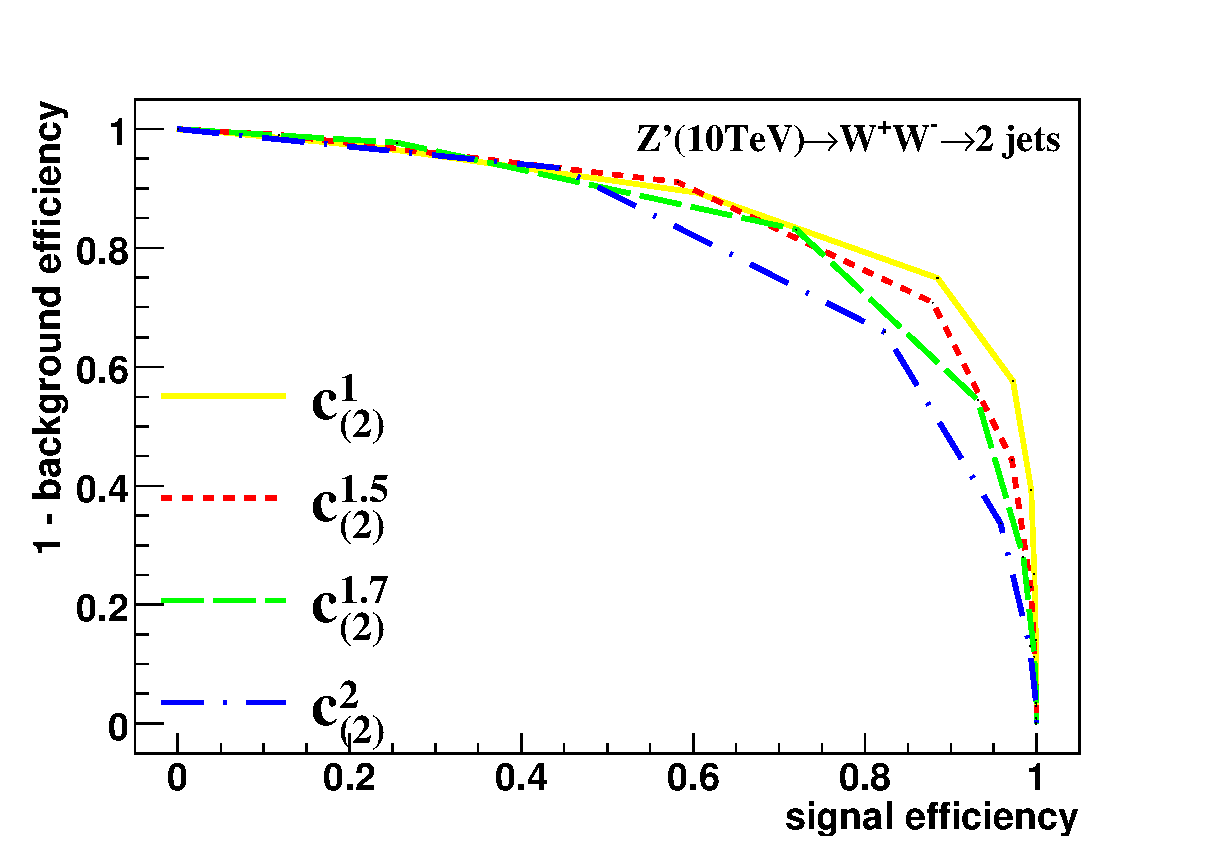
\includegraphics[width=0.43\textwidth]{figs/cluster_r010_c_variable_10tev_04_eff.eps}
   }
   \subfigure[20TeV] {
   \includegraphics[width=0.43\textwidth]{figs/cluster_r010_c_variable_20tev_04_eff.eps}
   }
   \subfigure[40TeV] {
   \includegraphics[width=0.43\textwidth]{figs/cluster_r010_c_variable_40tev_04_eff.eps}
   }

\end{center}
\caption{Signal efficiency versus background rejection rate using $c_2^{(1)}$,$c_2^{(1.5)}$,$c_2^{(1.7)}$,$c_2^{(2)}$ in different energies of collision for the cell size of  20$\times$20(cm$\times$cm).The energies of collision at (a)5, (b)10, (c)20, (d)40TeV are shown here.}
\label{fig:cluster_r010_c_variable}
\end{figure}

%25bins
\begin{figure}
\begin{center}
   \subfigure[5TeV] {
   \includegraphics[width=0.43\textwidth]{figs/cluster_r009_c_variable_5tev_04_eff.eps}\hfill
   }
   \subfigure[10TeV] {
   \includegraphics[width=0.43\textwidth]{figs/cluster_r009_c_variable_10tev_04_eff.eps}
   }
   \subfigure[20TeV] {
   \includegraphics[width=0.43\textwidth]{figs/cluster_r009_c_variable_20tev_04_eff.eps}
   }
   \subfigure[40TeV] {
   \includegraphics[width=0.43\textwidth]{figs/cluster_r009_c_variable_40tev_04_eff.eps}
   }

\end{center}
\caption{Signal efficiency versus background rejection rate using $c_2^{(1)}$,$c_2^{(1.5)}$,$c_2^{(1.7)}$,$c_2^{(2)}$ in different energies of collision for the cell size of  5$\times$5(cm$\times$cm).The energies of collision at (a)5, (b)10, (c)20, (d)40TeV are shown here.}
\label{cluster_r009_c_variable}
\end{figure}

%25bins
\begin{figure}
\begin{center}
   \subfigure[5TeV] {
   \includegraphics[width=0.43\textwidth]{figs/cluster_r012_c_variable_5tev_04_eff.eps}\hfill
   }
   \subfigure[10TeV] {
   \includegraphics[width=0.43\textwidth]{figs/cluster_r012_c_variable_10tev_04_eff.eps}
   }
   \subfigure[20TeV] {
   \includegraphics[width=0.43\textwidth]{figs/cluster_r012_c_variable_20tev_04_eff.eps}
   }
   \subfigure[40TeV] {
   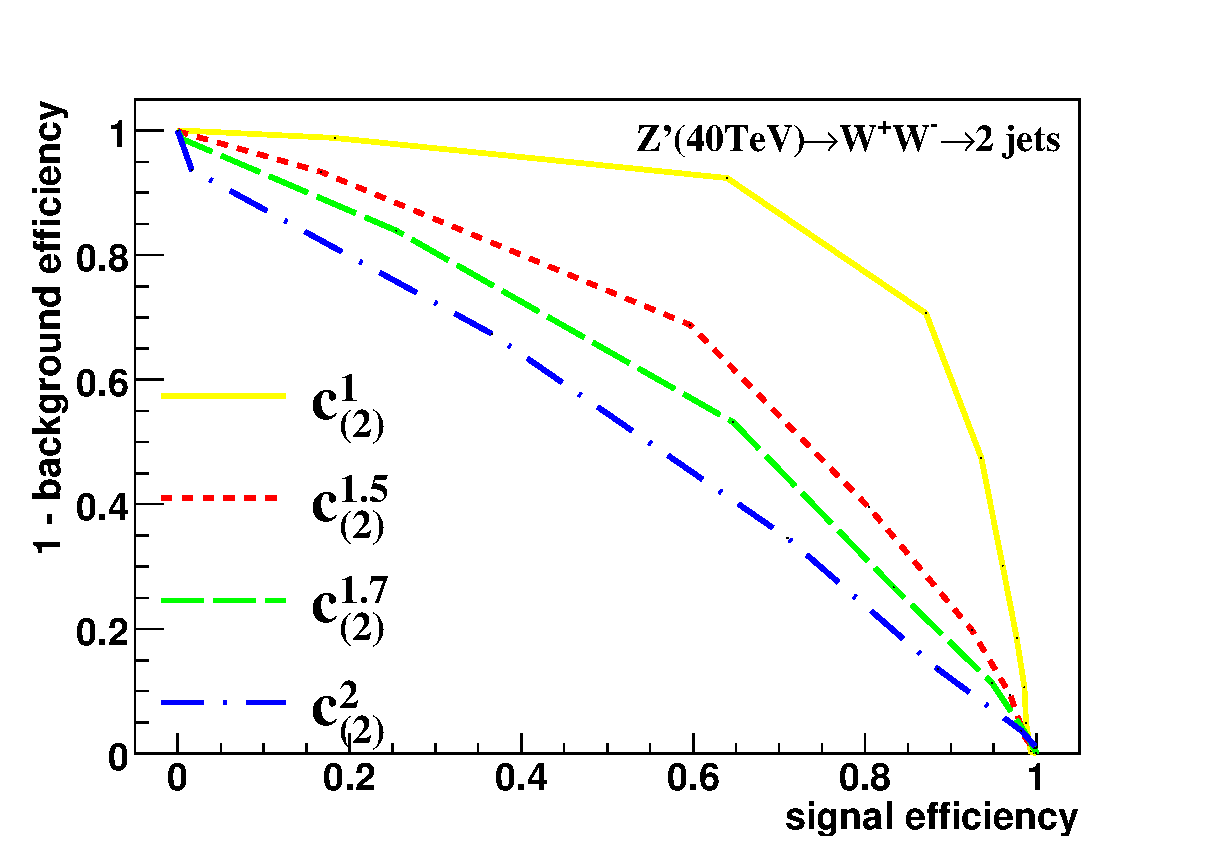
\includegraphics[width=0.43\textwidth]{figs/cluster_r012_c_variable_40tev_04_eff.eps}
   }

\end{center}
\caption{Signal efficiency versus background rejection rate using $c_2^{(1)}$,$c_2^{(1.5)}$,$c_2^{(1.7)}$,$c_2^{(2)}$ in different energies of collision for the cell size of  1$\times$1(cm$\times$cm).The energies of collision at (a)5, (b)10, (c)20, (d)40TeV are shown here.}
\label{cluster_r012_c_variable}
\end{figure}
\end{document}

